\documentclass{article}

\usepackage{lipsum}
\usepackage[nocheck]{fancyhdr}
\usepackage{graphicx}
\usepackage[T1]{fontenc}
\usepackage[scaled]{helvet}
\usepackage{titlesec}

\renewcommand\familydefault{\sfdefault}

% Define the indent size for subsections
\newlength{\subsecindent}
\setlength{\subsecindent}{1.5em}

% Define the format for subsection titles
\titleformat{\subsection}
  {\normalfont\bfseries}
  {\hspace{\subsecindent}\thesubsection}
  {1em}
  {}

% Define the format for subsubsection titles
\titleformat{\subsubsection}
  {\normalfont\itshape}
  {\hspace{2\subsecindent}\thesubsubsection}
  {1em}
  {}

% Remove the index from subsubsection
\renewcommand{\thesubsubsection}{\roman{subsubsection}}







\pagestyle{fancy}
\rhead{Management Software for Informal Businesses}
\rfoot{St. Paul's University}


\begin{document}
\setlength{\parindent}{10pt}
\renewcommand{\baselinestretch}{1.5}
\setlength{\parskip}{0.5em}
\setlength{\textwidth}{6.5in}
\setlength{\textheight}{9.5in}
\setlength{\topmargin}{-0.5in}

\thispagestyle{empty}
\begin{center}
	{\bfseries\huge
		St. Paul's University \\
		BAR 4102A \\
		IT Business Research Project \\
		Charles Kamiri  \\
		BOBITNRB200621 \\ [60pt]
	}

\emph{Management Software for Informal Businesses}
\end{center}
\newpage


% Table of Contents
\thispagestyle{empty}
\renewcommand{\contentsname}{Table of Contents}
\tableofcontents
\newpage


% Introduction
\section{Introduction}
\subsection{Background}
\paragraph{}
Informal businesses, also known as micro, small, and medium enterprises (MSMEs), are a critical component of the global economy. These businesses provide employment opportunities and contribute to economic growth in many developing countries.


\subsection{Problem Statement}
\paragraph*{}
HoIver, most informal businesses face several challenges, such as limited access to financial resources, lack of business skills, and poor record-keeping practices. These challenges hinder the growth and sustainability of these businesses, limiting their potential to contribute to the economy.

\subsection{Objectives}
\paragraph*{}
To address these challenges, I propose the development of a management software specifically designed for informal businesses. The software aims to provide a simple, affordable, and accessible solution to help these businesses manage their operations effectively. The software will offer features such as inventory management, sales tracking, financial management, and customer relationship management. With these features, informal businesses will be able to keep accurate records, make informed decisions, and improve their profitability.

\subsection{Justification}
\paragraph*{}
Our proposed management software is designed to be user-friendly, affordable, and accessible to all types of informal businesses, regardless of their level of technical expertise. I believe that this software can have a significant impact on the growth and sustainability of informal businesses, leading to more significant contributions to the economy.

\subsection{Limitations}
\paragraph*{}
Limited access to technology: Many informal businesses may not have access to the necessary technology, such as computers or smartphones, to use the management software effectively. This could limit the potential reach and impact of the software.

\paragraph*{}
Limited data availability: Informal businesses may not have access to the same level of data as formal businesses, making it more difficult to develop accurate and reliable management software. This could result in incomplete or inaccurate information being used to make business decisions.

\paragraph*{}
Limited financial resources: Many informal businesses operate on very limited budgets, which may make it difficult for them to afford the cost of the software or the hardware required to use it.

\paragraph*{}
Limited technical expertise: Informal business owners may not have the technical expertise required to use the management software effectively, which could limit its usefulness and adoption.

\paragraph*{}
Resistance to change: Some informal businesses may be resistant to adopting new technology or changing their existing business practices, which could limit the adoption and effectiveness of the management software.

\paragraph*{}
Limited scalability: If the management software is not designed to be scalable, it may not be able to handle the growing needs of businesses as they expand, potentially limiting its usefulness over time.

\paragraph*{}
Lack of integration with existing systems: If the management software is not designed to integrate with existing systems or software used by informal businesses, it may not be used effectively or may require additional work to use alongside existing tools.
\newpage


% Literature Review
\section{Literature Review}
\paragraph*{}
Management software for informal businesses has gained attention in recent years due to its potential to improve business performance. Several studies have explored the use of management software by informal businesses, identifying its benefits and challenges.

\paragraph*{}
A study by Akter and colleagues (2019) examined the adoption of management software among informal businesses in Bangladesh. The study found that the use of software significantly improved business performance, including sales growth and profitability. HoIver, the study also identified several challenges, including the lack of technical expertise and infrastructure.

\paragraph*{}
Similarly, a study by Fuchs and colleagues (2021) examined the impact of a mobile-based management system on microenterprises in Tanzania. The study found that the system improved businesses' ability to manage inventory and finances, leading to increased sales and profitability. The study also highlighted the importance of user-friendly software and training to overcome barriers to adoption.

\paragraph*{}
Another study by Yumusak and colleagues (2021) investigated the factors influencing the adoption of management software by informal businesses in Turkey. The study found that businesses Ire more likely to adopt software if they perceived it to be useful, easy to use, and compatible with their existing systems. The study also highlighted the importance of social networks in promoting software adoption among informal businesses.

\paragraph*{}
The research revieId in this literature review suggests that management software can significantly improve the performance of informal businesses. HoIver, the adoption of software by informal businesses faces several challenges, including technical expertise, infrastructure, user-friendliness, and compatibility with existing systems. Addressing these challenges through training and social networks can help to promote the adoption of management software by informal businesses.


\newpage

\section{Methodology}
\subsection{Overview}

This section contains a describption of the methodology that will be followed to develop our software system. The methodology is based on the agile software development approach, which emphasizes collaboration, flexibility, and responsiveness to change. I will divide the development process into several phases, each of which whill involve different activities and deliverables.

\subsubsection{Purpose}
The purpose of this project is to develop a management software that can help informal businesses to manage their daily operations and grow their business. The software will provide features such as inventory management, sales tracking, expense tracking, customer management, and reporting.

\subsubsection{Target Audience}
The target audience for this software is informal businesses such as small shops, food vendors, and service providers. These businesses often lack the resources and expertise to manage their operations efficiently and could benefit from a simple and easy-to-use management software.

\subsubsection{Scope}
The scope of this project includes developing a web-based management software that can be accessed from any device with an internet connection. The software will include the following features:

\begin{itemize}
    \item Inventory management: Keep track of products, quantities, and prices.
    \item Sales tracking: Record sales transactions and generate sales reports.
    \item Expense tracking: Record expenses and generate expense reports.
    \item Customer management: Store customer information and purchase history.
    \item Reporting: Generate reports on sales, expenses, and inventory.
\end{itemize}
\newpage


\subsection{Requirements Gathering}

\subsubsection{User Needs}
\paragraph*{}
To understand the needs of the target audience, the following data will be collected:

\begin{itemize}
    \item Demographic information: Age, gender, location, and occupation of the target audience.
    \item Business information: Types of products or services offered, current challenges faced by the business, and current methods of managing operations.
\end{itemize}

The data will be collected through surveys and interviews with informal business owners.

\subsubsection{User Behavior}
To understand how the target audience currently manages their operations and how they may use the software, the following data will be collected:

\begin{itemize}
    \item Inventory data: Types of products, quantities, and prices.
    \item Sales data: Transactions, customer information, and payment methods.
    \item Expense data: Types of expenses, amounts, and frequency.
    \item Customer data: Information on customer demographics, purchase history, and loyalty.
\end{itemize}

The data will be collected through the software itself, which will track and store the relevant information.

\subsubsection{Performance Metrics}
To ensure that the software is meeting the needs of the target audience and improving their operations, the following performance metrics will be collected:

\begin{itemize}
    \item User engagement: Number of users, frequency of use, and time spent on the software.
    \item Software performance: Speed, reliability, and availability of the software.
    \item Business performance: Improvement in sales, reduction in expenses, and growth of the business.
\end{itemize}

The data will be collected through the software itself and analyzed using data analysis tools. 

\subsubsection{Tools}
To collect and analyze the data, the following tools will be used:

\begin{itemize}
    \item Survey and interview tools: Google Forms and Zoom.
    \item Data analysis tools: Excel and Tableau.
\end{itemize}

Google Forms and Zoom will be used to conduct surveys and interviews with informal business owners. The data collected will be analyzed using Excel and Tableau, which will help identify patterns and insights from the data.
\newpage


\subsection{Architectural Framework}

\paragraph*{}
A model-driven approach will be utilized to design the software system's architecture. I will use UML (Unified Modeling Language) to create high-level diagrams that capture the system's structure and behavior. I will also use design patterns to guide our design decisions and ensure that our software system is scalable, maintainable, and extensible.

\paragraph*{}
The architectural design consists of several components, including the user interface, application logic, and database. The user interface will be designed using a responsive design approach, which will ensure that the software system is accessible and usable across different devices and platforms. The application logic will be designed using a modular approach, which  will allow for the breaking down the system into smaller, more manageable components. The database will be designed using a relational database management system (RDBMS), which will provide a flexible and efficient way to store and retrieve data.

\paragraph*{}
The software architecture of our system is designed to provide a scalable and extensible framework for building complex software applications. The architecture is based on a layered approach, with each layer providing a specific set of functionality and services.

\paragraph*{}
The architectural framework of our system is based on the Model-View-Controller (MVC) design pattern. This design pattern separates the application logic into three distinct components:

\begin{itemize}
\item \textbf{Model}: This component represents the data and the business logic of the application.
\item \textbf{View}: This component represents the user interface of the application.
\item \textbf{Controller}: This component acts as the intermediary between the Model and the View, and handles user input and business logic.
\end{itemize}

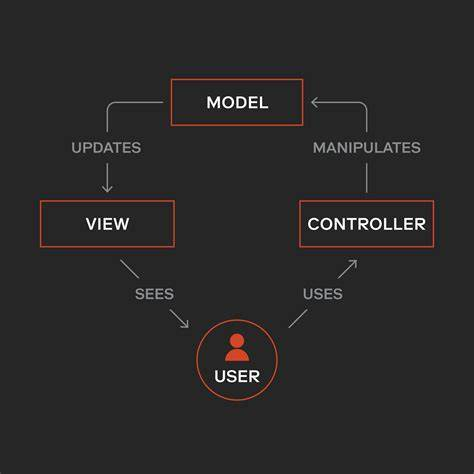
\includegraphics[width=0.5\textwidth]{mvc.jpeg}



By separating these components, we can achieve greater modularity, maintainability, and flexibility in our codebase.

\subsection{Component Overview}

Our system consists of several components, each providing a specific set of functionality:

\subsubsection{Database Layer}

The database layer is responsible for managing the persistence of data in our system. We use a relational database management system (RDBMS) to store and retrieve data, and we use an Object-Relational Mapping (ORM) framework to map the database schema to our application's data model.


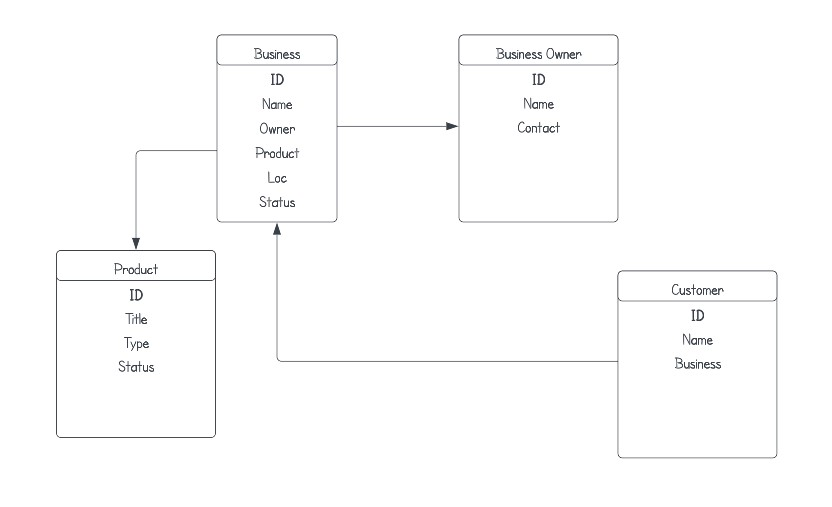
\includegraphics[width=0.9\textwidth]{db_schema.jpg}
\subsubsection{Business Logic Layer}

The business logic layer is responsible for implementing the core functionality of our application. This layer contains the Model component of the MVC architecture, and is responsible for managing the data and the application logic.

\subsubsection{Presentation Layer}

The presentation layer is responsible for providing the user interface of our application. This layer contains the View and Controller components of the MVC architecture, and is responsible for rendering the data and handling user input.

\subsubsection{Integration Layer}

The integration layer is responsible for integrating our system with other external systems and services. This layer provides interfaces for communicating with other systems, and handles data transformation and mapping between our system and external systems.

\subsubsection{Infrastructure Layer}

The infrastructure layer is responsible for providing the underlying infrastructure and services required to run our system. This layer includes components such as web servers, load balancers, and network infrastructure.


\subsection{Implementation}

The third phase of our development process is implementation. I will use a test-driven development (TDD) approach to implement the software system's components. TDD involves writing automated tests for each component before writing the code for the component. This approach ensures that the software system is reliable, maintainable, and had good test coverage.

I will employ several programming languages and frameworks to implement the software system's components. The user interface will be implemented using the React framework which compiles to HTML, CSS and JavaScript, and the application logic to be implemented using Java and the Java Spring Boot web framework. The database will be implemented using PostgreSQL, a popular open-source RDBMS.

\subsection{Testing}

The fourth phase of the development process is testing. I will use various testing techniques such as unit testing, integration testing, and acceptance testing to test the software system's components. I will also employ manual testing to ensure that the software system is user-friendly and meets the stakeholders' needs and requirements.

A continuous integration and continuous deployment (CI/CD) approach to automate the testing and deployment process  will be implemented. The use of GitHub Actions to automate the testing and deployment process, will allow for quick detection and fixation of any issues that may arise during the development process will also be used.

\subsubsection{Unit Testing}
\paragraph*{}
Unit testing is a type of software testing where individual components of the system are tested in isolation to ensure that they work as expected.

\paragraph*{Frontend (React)}
\paragraph*{}
The frontend components will be tested using the Jest testing framework. Jest is a popular testing framework for React applications, and provides a set of tools for testing React components. Jest also provides a set of tools for mocking and stubbing, which will be used to mock the backend API.

\paragraph*{Backend (Java)}
\paragraph*{}
The backend components will be tested using the JUnit testing framework. JUnit is a popular testing framework for Java applications, and provides a set of tools for testing Java classes and methods. JUnit also provides a set of tools for mocking and stubbing, which will be used to mock the database.

\subsubsection{Integration Testing}
\paragraph*{}
Integration testing is a type of software testing where the components of the system are tested as a group to ensure that they work together as expected.

\paragraph*{}
Integration testing will be an important part of the testing phase for the management software for informal businesses. I will write integration tests to ensure that the React frontend, Java Spring backend, and Postgres database are all working together as expected. For example, I will write tests that simulate user interactions with the frontend and ensure that the data is correctly stored in the database via the backend API. I will also test the communication between the frontend and backend to ensure that requests and responses are being sent and received correctly. These integration tests will help catch any issues that may arise from the interactions between our different components and ensure that the system is working as a cohesive whole.

\subsubsection{Acceptance Testing}
\paragraph*{}
Acceptance testing is critical to ensure that the management software for informal businesses meets the needs and requirements of the stakeholders. I will write acceptance tests that simulate typical user interactions with the software, such as creating a new business account, adding products or services, and generating financial reports. I will also ensure that the system is user-friendly and easy to navigate. These tests will help to validate that the system is meeting the stakeholders' needs, and ensure that it is intuitive and easy to use. Additionally, I will use any feedback received from stakeholders during acceptance testing to iterate and improve the software before it is released.

\subsubsection{Manual Testing}
\paragraph*{}
Manual testing will be a crucial part of ensuring that the management software for informal businesses is user-friendly and meets the stakeholders' needs. I will manually test the software to validate that it is easy to navigate, that users can easily find the features they need, and that the system responds appropriately to user inputs. Additionally, I will test the software's performance to ensure that it can handle the expected user load without lagging or crashing. Manual testing will allow for easy identification of any issues that may have been missed in automated testing and ensure that the system is easy to use and reliable.

\subsection{Maintenance}

The final phase of the development process is maintenance. I will use various techniques such as bug tracking, performance monitoring, and user feedback to maintain the software system. I will also use a DevOps approach to ensure that the software system is reliable, scalable, and secure. I will utilize cloud hosting services such as Amazon Web Services (AWS) and Google Cloud Platform (GCP) to deploy and manage the software system.

Overall, the methodology will ensure and guarantee the delivery of a high-quality software system that meets the stakeholders' needs and requirements. I will follow a collaborative and flexible approach that will allow for quick response to changes and ensure that the software system is reliable, maintainable, and scalable.

\newpage


% References
\section{References}
\renewcommand{\refname}{}
\begin{thebibliography}{10}
	\bibliographystyle{apalike}
	% Add references here
	\bibitem{ref1}
	Akter, S., Islam, S., \& Ahsan, M. (2019). Adoption of management software among microenterprises in Bangladesh: An empirical study. Information Development, 35(2), 265-280.

	\bibitem{ref2}
	Fuchs, C., Huesing, T., \& Schäfer, M. (2021). Mobile-based management systems for informal businesses in Tanzania: Effects on business performance and adoption barriers. Journal of Business Research, 129, 496-507.

	\bibitem{ref3}
	Yumusak, I. G., Coskun, Y., \& Ozkan-Ozen, Y. D. (2021). Factors influencing adoption of management software among small businesses: The case of Turkey. Journal of Enterprise Information Management, 34(1), 27-45.

\end{thebibliography}
\end{document}